\subsection{Third dosage label (Collins et al.\ 2022 rCNV scores): the depletion survives UTR-length matching}
We then used the pHaplo and pTriplo scores of Collins et al.\ (Zenodo 6347673; 18,641 genes), which are estimated from rare CNVs in about 950,000 people. We noted in advance that the model uses gene features that include gnomAD constraint, so this label is only partly independent of LOEUF. Same 43 miRNAs and controls; the script was committed before it was run (\texttt{collins\_dosage}). Gates passed: 95.4\% coverage, and TargetScan conserved top-200 sets have higher pHaplo than random UTR genes (36/2, $p=2.7\times10^{-9}$).
\begin{table}[h]\centering\small\begin{tabular}{lcccc}\hline Pre-registered test (CNN lower) & wins/losses & $p$ & median diff. & verdict\\\hline
D1 pHaplo vs uniform & 43/0 & $1.1\times10^{-13}$ & -0.131 & CONFIRMED \\
D2 pHaplo vs expression-matched & 43/0 & $1.1\times10^{-13}$ & -0.099 & CONFIRMED \\
D3 pHaplo vs UTR-length-matched & 38/5 & $1.2\times10^{-7}$ & -0.038 & CONFIRMED \\
T3 pTriplo vs UTR-length-matched & 42/1 & $5.0\times10^{-12}$ & -0.054 & CONFIRMED \\
\hline\end{tabular}\caption{Collins 2022 dosage scores of CNN top-200 sets, 43 miRNAs.}\label{tab:collins}\end{table}
All four hypotheses are confirmed, including against UTR-length-matched sets for both haploinsufficiency and triplosensitivity (Figure~\ref{fig:collins}). Across the three labels the picture is: LOEUF and the rCNV scores support depletion beyond UTR length; the sparse ClinGen curation does not. Because the rCNV model shares features with LOEUF, it is not a clean third vote, and the finding stays at the strength of its weakest independent test. The later locked random-weight falsifier failed, so these descriptive dosage-label contrasts are not evidence that trained CNN weights caused the pattern.
\begin{figure}[h]\centering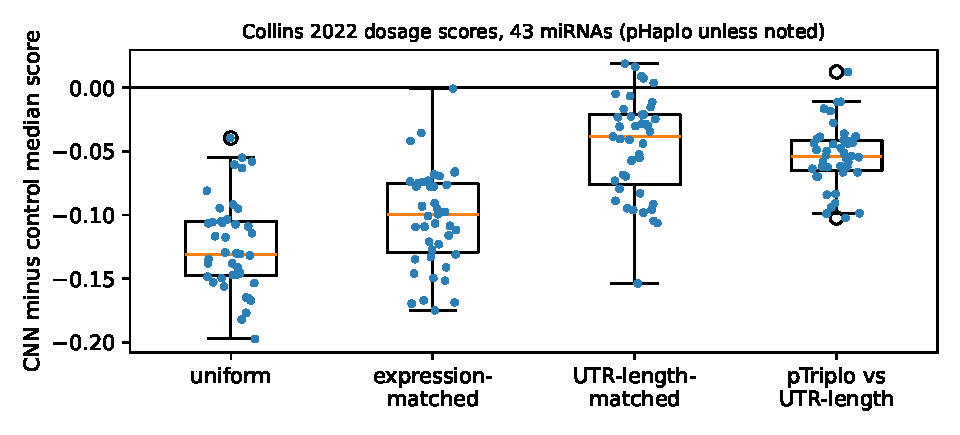
\includegraphics[width=0.66\linewidth]{figs/fig_collins.pdf}
\caption{Per-miRNA difference between CNN top-200 and control median dosage score (negative = CNN less dosage-sensitive).}\label{fig:collins}\end{figure}
